4. Для нахождения области определения данной функции необходимо решить неравенство\\ $\cfrac{|x-1|(x+3)(x^2+8x+15)}{x^2+x-2}\geqslant0\Leftrightarrow
\cfrac{|x-1|(x+3)^2(x+5)}{(x-1)(x+2)}\geqslant0.$ Применив метод интервалов, найдём ответ:
\begin{figure}[ht!]
\center{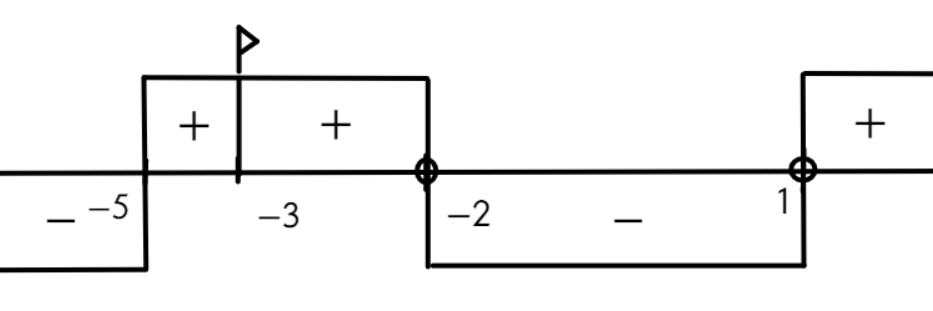
\includegraphics[scale=0.35]{isl4.png}}
\end{figure}
$x\in[-5;-2)\cup(1;+\infty).$\\
